%File: algorithm.tex
%Date: Sun Nov 17 23:30:40 2013 +0800
%Author: Yuxin Wu <ppwwyyxxc@gmail.com>

\section{Algorithm and Implementation}

We presented a prototype system based on MFCC as acoustic features, and
GMM as our recognition model.

\subsection{MFCC}
MFCC (Mel-frequency Cepstral Coefficient) is a representation of the short-term power spectrum of a sound,
based on a linear cosine transform of a log
power spectrum on a nonlinear mel-scale of frequency \cite{mfcc} .
MFCC is the mostly widely used features in Automatic Speech Recognition(ASR), and it can also be
applied to Speaker Recognition task.

The process to extract MFCC feature is as followed:
\begin{figure}[H]
  \centering
  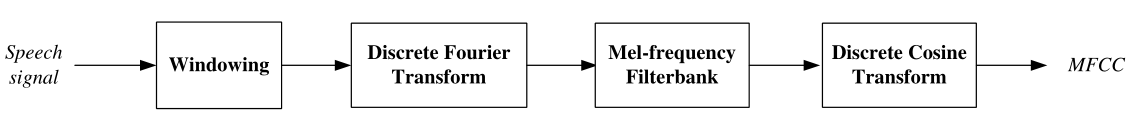
\includegraphics[width=\textwidth]{res/MFCC.png}
\end{figure}

First, the input speech should be divided into successive short-time frames of length $L$,
neighboring frames shall have overlap $R$. We choose $L = 20ms  $ ans $ R = 10 ms$.
Those frames are then windowed by Hamming Window, as shown in \figref{frames}
\begin{figure}[H]
  \centering
  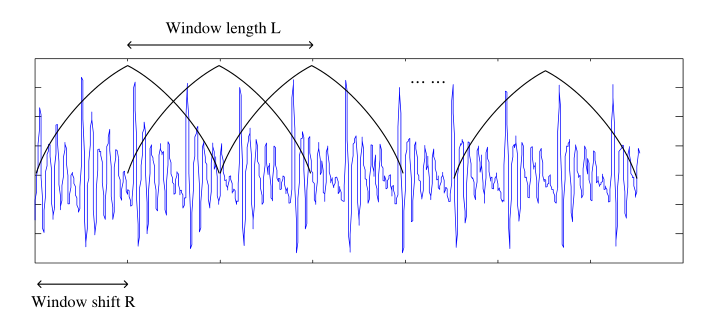
\includegraphics[width=0.7\textwidth]{res/frames.png}
  \caption{Framing and Windowing \label{fig:framming}}
\end{figure}

Then, We perform Discrete Fourier Transform (DFT) on windowed signals to compute their spectrums.
For each of $N$ discrete frequency bands we get a complex number $X[k]$ representing
magnitude and phase of that frequency component in the original signal.

Considering the fact that human hearing is not equally sensitive to all frequency bands, and especially, it has lower resolution at higher frequencies.
Scaling methods like Mel-scale and Bark-scale are aimed at scaling the frequency domain to fit human auditory perception better.
They are approximately linear below 1 kHz and logarithmic above 1 kHz.
\begin{figure}[H]
  \centering
  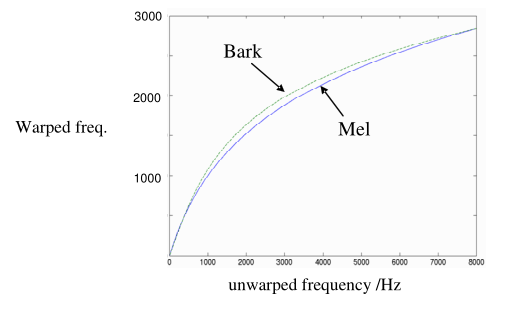
\includegraphics[width=0.6\textwidth]{res/mel-scale.png}
\end{figure}

In MFCC, Mel-scale is applied on the spectrums of the signals. The expression of Mel-scale warpping is as followed:
\[ M(f) = 2595 \log_{10}(1 + \dfrac{f}{700}) \]

\begin{figure}[H]
  \centering
  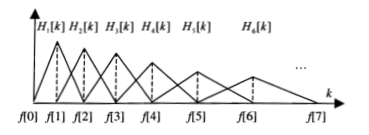
\includegraphics[width=0.5\textwidth]{res/bank.png}
  \caption{Filter Banks (6 filters) \label{fig:bank}}
\end{figure}
Then,  we appply the bank of filters according to Mel-scale on the spectrum,
calculate the logarithm of energy under each bank by $E_i[m] = \log (\sum_{k=0}^{N-1}{X_i[k]^2 H_m[k]}) $ and apply Discrete
Cosine Transform (DCT) on $E_i[m](m = 1, 2, \cdots M) $ to get an array $c_i $:
\[ c_i[n] = \sum_{m=0}^{M-1}{E_i[m]\cos(\dfrac{\pi n}{M}(m - \dfrac{1}{2}))} \]

Usually, the first 13 terms in $c_i $ is used as features for future training.

\subsection{GMM}

For all feature vectors, we cluster them into a small number of classes.
Gaussian Mixture Model (GMM) can be used to calculate the probability that the class is generated by a given input modal.
The modal with maximum conditional probability is picked out as the result.
